\section{Data Wrangling at Scale}\label{sec:architecture}
As mentioned above, in the designed architecture a logical separation between platform and corporate services has been imposed. This structure is conceived to make the architecture flexible and adaptable to different deployment scenarios. 
In what follows, the main components and interaction of the platform are presented. 

Figure~\ref{fig:wrangler} shows a component diagram of our wrangling solution with component interactions and information flows. 
The image presents the most general case, where the data set to be transformed is genuine Big Data and, for this reason, it is managed by the corporate services. 
In this scenario, components from all logical areas are involved; we have on the left a corporate component called \textit{Sampler} , the \textit{Summarizer} and the \textit{Engine} that are the components that are entrusted of creating the (reduced) working data set to be used to define the transformations, of providing a set of suggestions for the table annotation process based on summaries of existing knowledge bases or previous annotations, and finally, of interacting with the \textit{Big Data Runtime} to carry out on a large scale the transformations defined by the user, respectively. 
\begin{figure}[t]
    \centering
    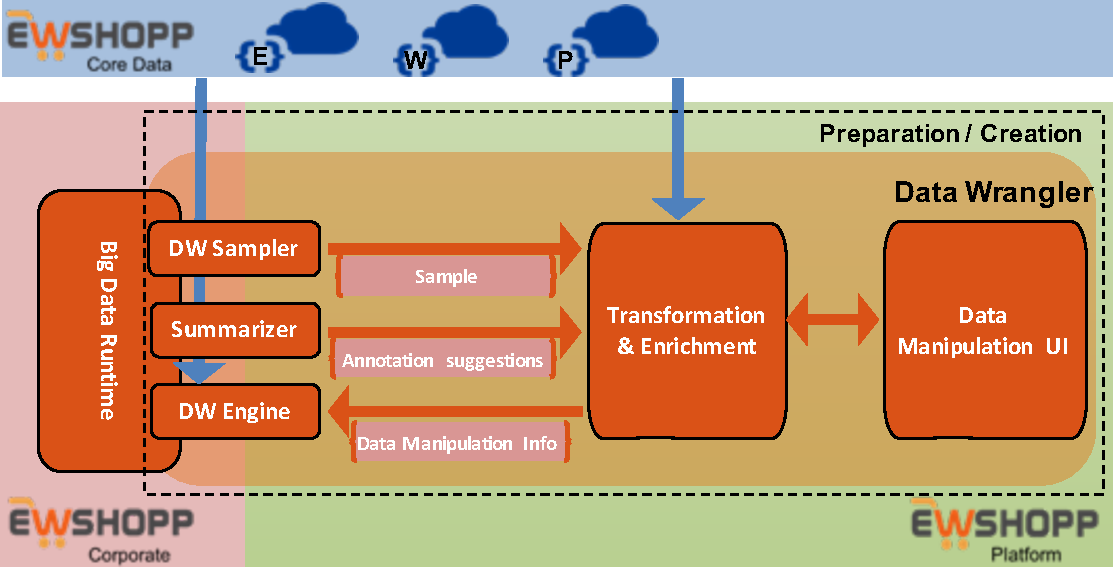
\includegraphics[width=\columnwidth]{figs/Wrangler.pdf}
    \caption{Data Wrangler's components and interactions}
    \label{fig:wrangler} 
\end{figure}  
The definition of the transformation pipeline, instead, is carried out using the platform services, depicted on the right side of the Figure. In particular, the user is supported in this task by a graphical manipulation interface, which in turn interacts with a \textit{Transformation and Enrichment} back-end service. This service has the twofold duty of executing the pipeline on the reduced data set, thus allowing the platform to be used as a standalone solution, and of interacting with the corporate services. In both cases, core data services support linking and extension capabilities. 

The architecture and components interactions within the Big Data Runtime are depicted in Figure~\ref{fig:big_data_runtime}. The \textit{System Orchestration} sub-component is used to define the high-level data flows that will be executed by \textit{Processing} tool. 
Such Data flows include the data wrangling pipelines but they may also incorporate pre- and post-processing steps, e.g, automatic obtaining of data, re-formatting, import to a data warehouse (enrichment database). The end result is a data flow that can be deployed as a Function as a Service (FaaS) computing service over a managed cluster of resources, which allows for easy integration with business processes and heterogeneous infrastructures (see Section~\ref{sec:bdr}).

For sake of clarity a high-level workflow is reported:
\begin{enumerate}
    \item A reduced data set (possibly complemented by profiling information) is created and passed to the \textit{Transformation and Enrichment} component.
    \item The user operates the \textit{Data Manipulation UI}, which also interacts with the Core Data services and \textit{Summarizer} to perform schema and entity linking, to extend the data with weather and events information.
    \item The application generates a self-contained machine-runnable pipeline of the user's operations which is eventually executed on the original data set by the \textit{Big Data Runtime}. 
\end{enumerate}

\begin{figure}[t]
    \centering
    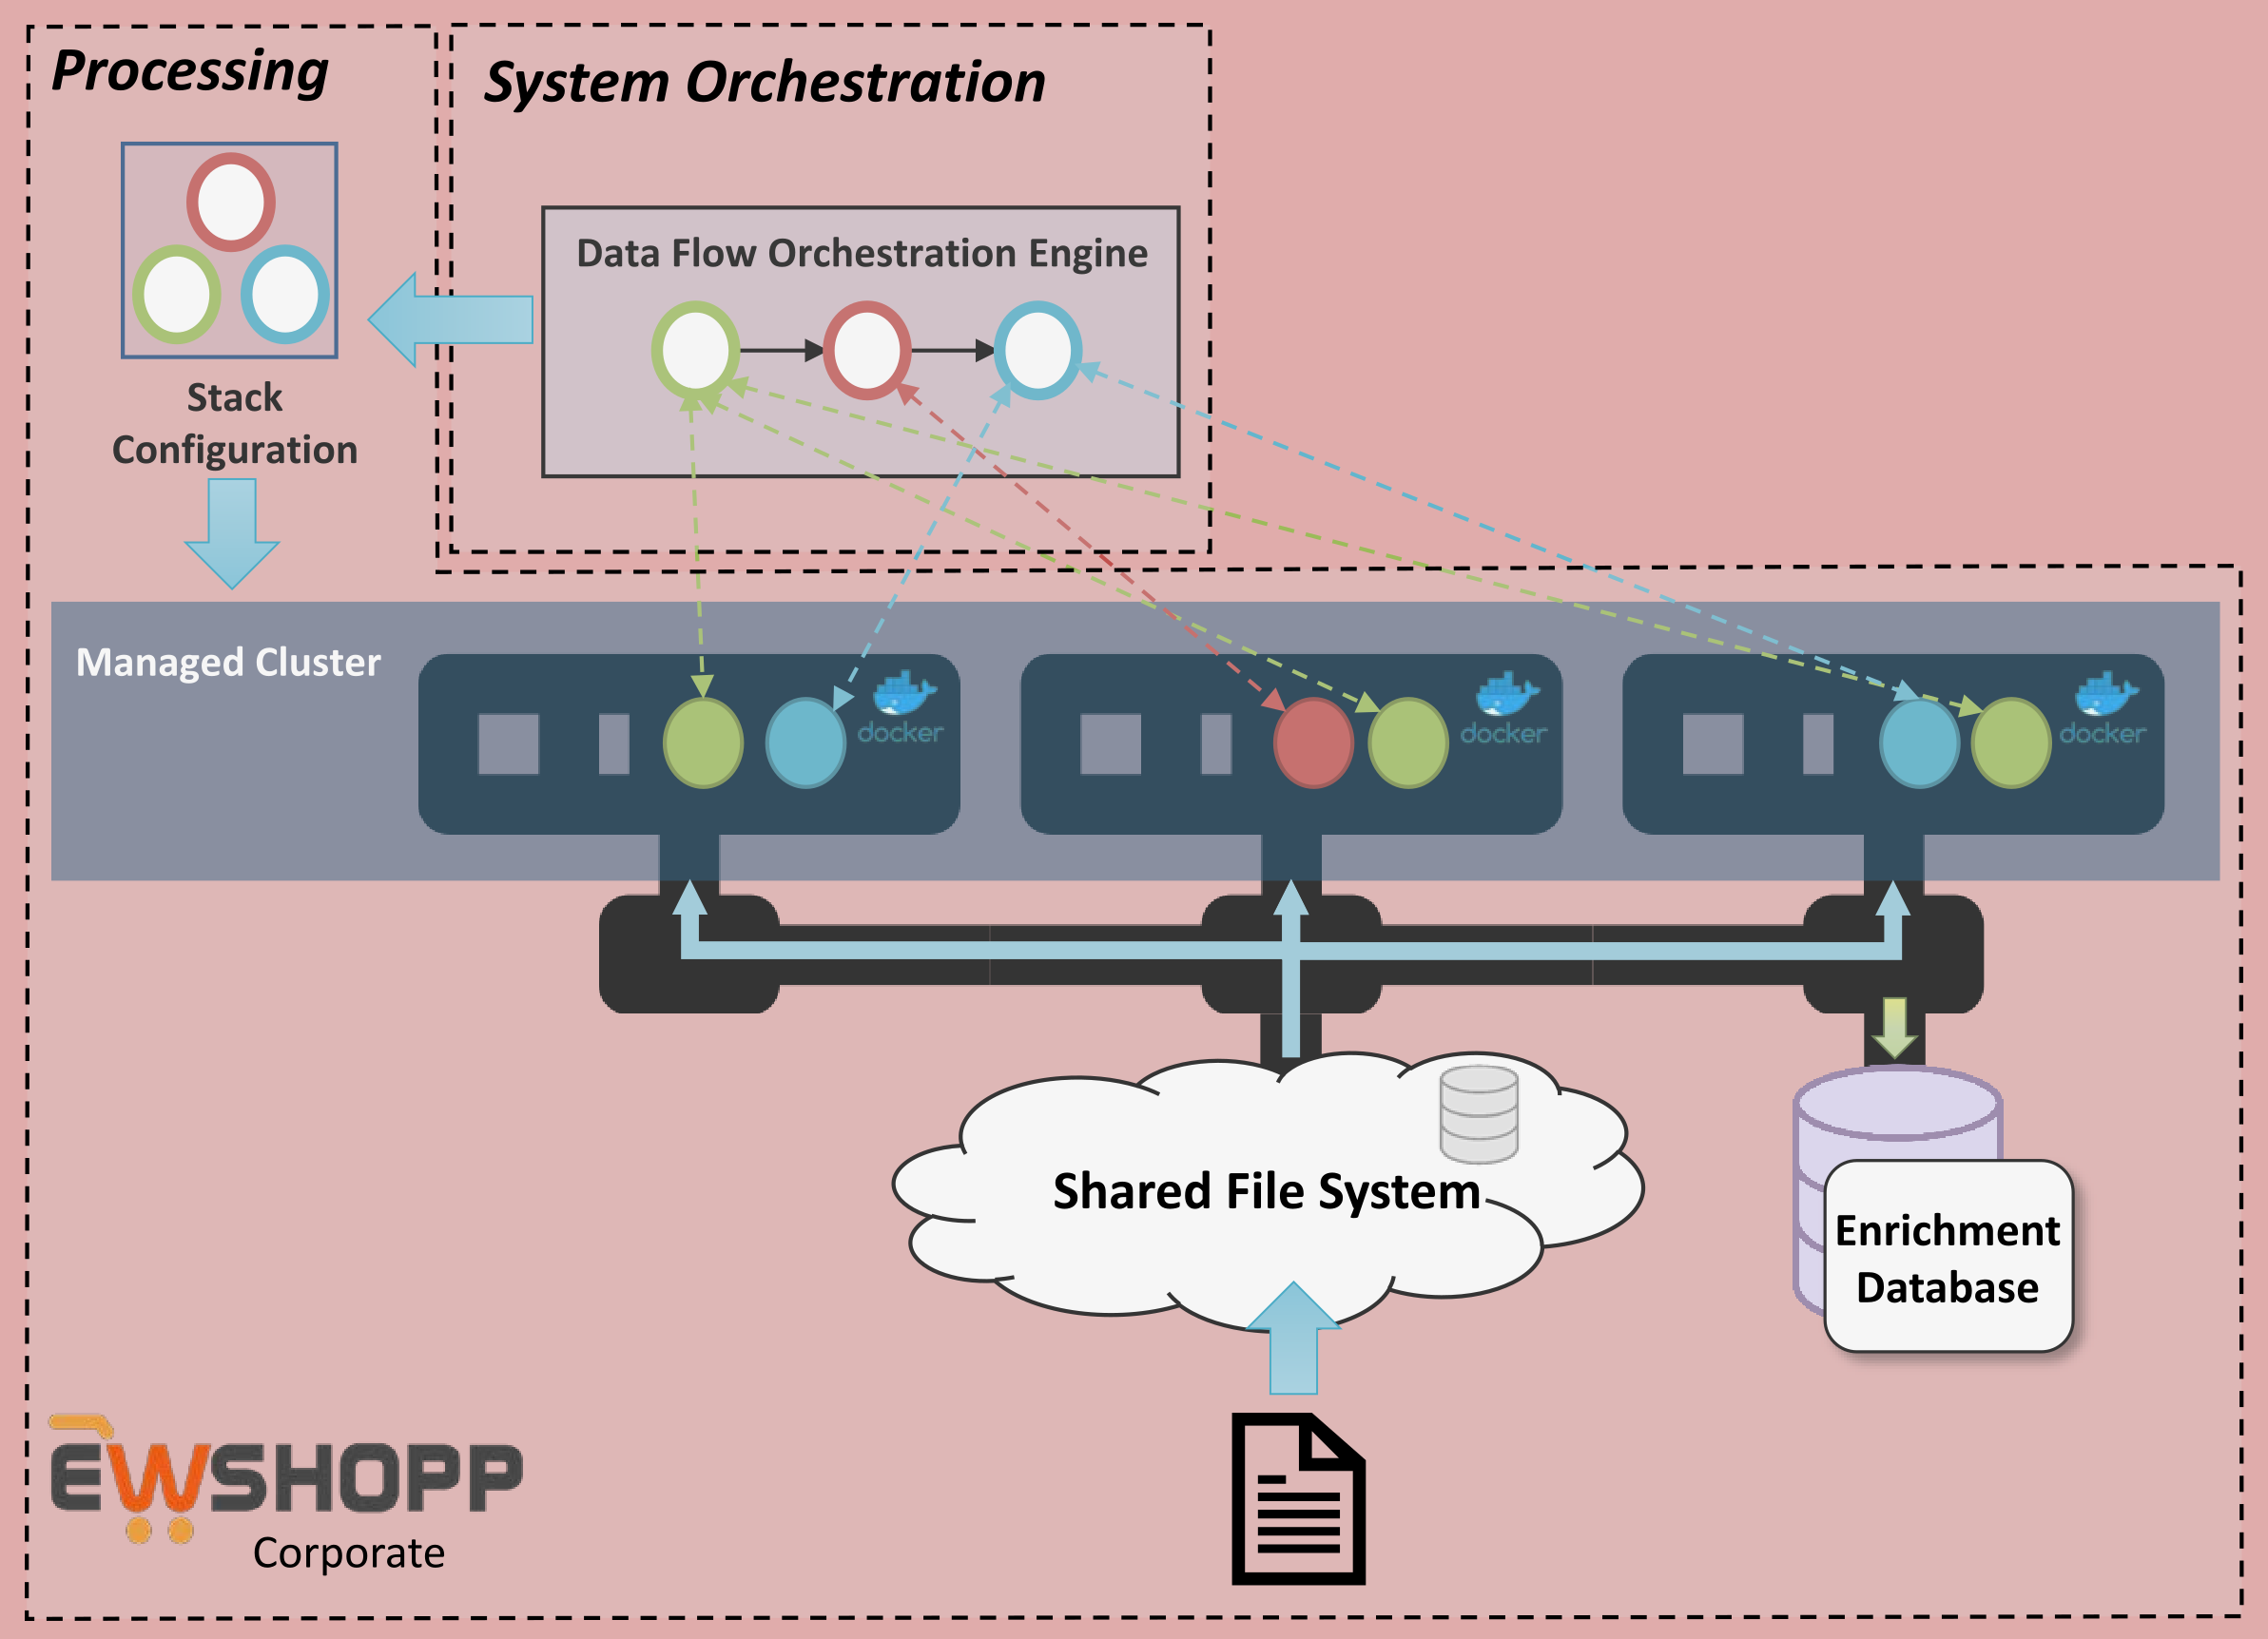
\includegraphics[ width=0.9\columnwidth]{figs/SACBD2018-Big-data-processing-engine.png}
    \caption{Big Data Runtime components interaction}
    \label{fig:big_data_runtime} 
\end{figure}  

The next two subsections detail the components and interactions of the proposed solution, highlighting which components are involved at design time and which at run time. 


\subsection{Platform services}

The Data Wrangler is a composite component built upon the DataGraft platform~\cite{roman2016datagraft}, extended with semantic enrichment and Big Data processing capabilities. DataGraft provides tools for cleaning and transformation of tabular data into RDF and graph generation mappings.
%featuring a composite architecture that follows the service-oriented architecture mandates. 
DataGraft comes with an interactive web application, named Grafterizer~\cite{sukhobok2016tabular}, which serves as a graphical interface helping platform users to transform data from a tabular format into a graph format. The transformation supports both cleaning and graph mapping steps. Transformation steps on rows (add, drop, filter, duplicate detection etc.), columns (add, drop, rename, merge etc.) and entire data set (sort, aggregate etc.) are provided together with visualization of the result after each step. The mapping to ontologies or vocabularies is performed on the cleaned-up data. 
%Moreover, the DataGraft is responsible for user-facing miscellaneous tasks such as user management, managing user assets (i.e., Enrichment Database endpoints, queries, transformation models) and enabling easy access to data.  

As mentioned, the EW-Shopp platform aims to support scalable data enrichment. Therefore, DataGraft and the transformation tool, Grafterizer, incorporate two sub-components called ASIA and ABSTAT. The components provide functionalities for the semantic enrichment of data tables and profiling of knowledge graphs, respectively. ASIA is meant to aid users in integrating business data and can be used to map the data schema to shared vocabularies/ontologies, or link data values to shared systems of identifiers, which enables the extraction of additional data from third-party sources and their fusion into the original tabular data. Schema-level and instance-level links are created by ASIA as annotations for the table. ABSTAT~\cite{palmonari2015abstat} is a tool to profile knowledge graphs represented in RDF based on linked data summarization mechanisms. The profiles extracted by ABSTAT describe the content of knowledge graphs, using abstraction (schema-level patterns) and statistics. Such profiles are exploited by ASIA to provide the user with suggestions in schema linking activity. 

\subsection{Corporate Services}\label{sec:bdr}

%We have introduced the platform components in the previous section, in this section we focus on the services of the corporate section. In the most general case, these components are physically distant from the platform components and interact with them via APIs. 
%In the early stages of pilot development, we do not rule out the possibility that the interaction between the components of the two logic areas can be carried out manually by means of one or more human users.  

%The Big Data Runtime (BDR) component's role in our solution is to perform batch data cleaning, integration, enrichment and data transformation at scale. 
%The objective of the pipeline is to eventually expose the data in a central database for performing analytics.

The Corporate services of the EW-Shopp solution are mainly responsible for the orchestration and execution of wrangling operations at scale. 
In particular, based on the user-defined data wrangling pipeline (cleaning, transformation, graph mapping, enrichment, and extension) declared on the sampled data, a so-called transformation model is created and transmitted to the corporate services in order to be applied to the full data set. Once there, the model is compiled into a self-contained executable Java archive (JAR) and executed as the main step of a larger process that is referred to as Data Flow.  
Data Flows are  extension of the data wrangling pipeline with pre- and post-processing actions. 
To serve as an example, a data flow coming from a business case of EW-Shopp is described below:
\begin{enumerate}
    \item Decompress data - large data set is delivered as a set of archives contain CSV files, which are stored in a shared file system of our private cloud.
    \item Split data in chunks for faster processing and horizontal scalability of inputs.
    \item Execute the data wrangling pipeline - Clean up, re-format, transform, map to ontology, and enrich the split data. 
    \item Import the resulting data set into the Enrichment database
\end{enumerate}



The System Orchestration component provides a high-level interface to handle and monitor a data flows, whereas the Processing component is in charge of carrying them out. From the technological point of view, data flows are compiled into a chain of Docker\footnote{https://www.docker.com/} containers that are in turn deployed and run through a Container Orchestration system (e.g., Kubernetes\footnote{\url{https://kubernetes.io/}}, Rancher\footnote{\url{https://rancher.com/}}) on a cluster of machines connected via an Ethernet fabric and mounting a shared filesystem (e.g., GlusterFS\footnote{\url{https://www.gluster.org/}}).
The implementation of a container-based solution has several benefits; for instance, it allows to decouple the data flow deployment from the particular stakeholder's hardware infrastructure also working in heterogeneous distributed environments. Furthermore, it guarantees flexible deployments, better resource utilization, and seamless horizontal scalability.  

 
%Each machine runs the Docker engine, so that Docker containers can be deployed. The particular virtual hardware allocated to each of the Docker container that implement the processing pipeline depends on the load and is configurable. The deployment of Docker containers is controlled at run time by the container orchestration system. 
Finally, for the sake of completeness, the following non secondary aspects of the execution of a data flow are presented>
\begin{description}
    \item[Deployment of the flow configuration] - the flow configuration contains the context information to be fed to each step that compose the data flow, as well as any additional hardware constraints for each step. These parameters are passed to the containers in the chain they are intended for. Notice that an extensible library implements the most common (parametrized) actions to be used in the definition of a data flow. Moreover, each action implements a common interface to guarantee both composability and observability. 
    
    %in order to handle the scale of data, the Big Data Runtime component has to be able to distribute the individual workflow steps over a cluster of virtual machines (VMs) or containers. The cluster can be deployed on the premise of the EW-Shopp platform user to maintain the confidentiality of their data. The cluster also needs to provide access to the input data to all members of the cluster, for example by deploying data are on a reachable network location or on a mounted shared file system.
    \item[Execution of the data flow] - The Processing component establishes a suitable deployment in terms of machines and resources to be used and starts the appropriate number of containers for each step of the flow.  Each of the steps consists in a set of containers that work independently and in parallel, and can be scaled up or down on demand if required. The communication between two consecutive steps of the chain, that is the handover of the partial results, occur through writing and reading from file system in a specific way, defined in the context information.
%a specific way: each container is given an input, work and output folder and the cluster configuration reflects those settings. %Race conditions between individual containers that implement the steps are solved using low-level file operations.
    \item[Data Storage] - The results of the data flow can be stored on disk or (more typically) imported to an Enrichment Database. The database serves as a single source of truth to be used, for example, to slice and dice the data to obtain a subset needed for analytics or machine learning jobs. 
    %The Big Data Runtime deploys the output of the data workflow in a central data storage solution, which is accessible through the network, or deployed on the same cluster. 
\end{description} 
%The tools and services for providing analytics and reporting functions consume the data produced by the data workflow executed by the Big Data Runtime (BDR) through the central database. 